La pluralité des mondes est un concept qui a lentement évolué au cours des âges. Dans l'antiquité grecque l'univers fini,
sphérique et géocentrique d'Aristote (384--322 av. JC) s'oppose à l'univers infini et discontinu des atomistes. Pour Épicure (v
342--270 av JC), il existe une pluralité de \textit{kosmoi}, portions de ciel contenant les corps célestes. Thalès (v 625-547
av. JC) pense que d'autres astres pourraient être similaires à la Terre. 

Le débat de la vie ailleurs et de l'existence d'autres planètes autour d'autres étoiles a animé la communauté scientifique
depuis l'antiquité. Le débat étant influencé par les convictions religieuses et les modèles du Système solaire en vigueur, il était
parfois dangereux d'émettre l'hypothèse que d'autres planètes ou d'autres formes de vies puissent exister, l'idée de la
pluralité des civilisations extraterrestres étant indissociable de la question de la pluralité des mondes physiques. D'autres auteurs au contraire, voyaient dans la pluralité des Mondes une preuve de l'immense pouvoir divin. Nous pouvons citer Jean d'Espagnet (1564-- c. 1637), président du parlement de Bordeaux et passionné d'Astronomie qui s'interrogeait sur l'existence de ces autres Mondes :
\begin{quote}
\og mesmes n'y auroit-il pas de l'apparence à croire que chaque globe est un monde, \& que tout autant qu'ils sont ce sont
autant de mondes, comme autant de fiefs qui relevent de l'Empire Divin, \& eternel, assis dans la vaste estenduë du Ciel
etherée, par le moyen duquel estans liez, comme par un lien commun, ils demeurent suspendus, \& que la vaste estenduë de
l'Univers est composée de toutes ces differentes natures?\fg 

--- Jean d'Espagnet, \textit{La Philosophie naturelle restablie en sa pureté}, 1651, p. 241 \cite{espagnet1651philosophie}
\end{quote}

Ces questions ont longtemps été des expériences de pensée, plus philosophiques et métaphysiques qu'étayées par de quelconques
observations. La découverte progressive du Système solaire et de la diversité des planètes qui la compose a permis de situer la
Terre dans un contexte un peu plus large. La question de la formation des planètes s'est alors posée. Remarquant la quasi-coplanarité des orbites du système Solaire, Kant (1755) puis Laplace (1796) ont introduit le concept de nébuleuse solaire
primitive, disque de matière duquel les planètes étaient issues. 

La ligne des glaces, séparation imaginaire au delà de laquelle l'eau est sous forme solide, s'intégrait bien dans ce concept et
dans le cas du système Solaire. En dessous de la ligne des glaces, nous formons des planètes essentiellement rocheuses, peu
massives. Au delà, la quantité de matière augmente, nous formons des géantes gazeuses. Durant leur formation, les planètes
n'évoluent pas beaucoup. La Nébuleuse Solaire de Masse Minimale (MMSN) a ainsi été inventée. Elle représente le disque le moins
massif qui est nécessaire pour former les planètes du système Solaire. Pour cela, la masse de chaque planète est dispersée
sur un anneau de matière entourant sa position orbitale.
Cette masse est corrigée pour tenir compte du gaz (abondant dans le cas de géantes comme Jupiter, mais rare pour une planète
comme la Terre). On obtient donc un profil de densité de surface en loi de puissance $\Sigma(R)=1700 * \frac{R}{1\unit{UA}}^{-\sfrac32}\unit{g/cm^2}$ \citep{
weidenschilling1977distribution, hayashi1981structure}.

La découverte de la première exoplanète\footnote{Planète orbitant autour d'une étoile autre que notre Soleil.}
\citep{wolszczan1992planetary} a quelque peu bouleversé le cadre théorique de la formation planétaire.

Bien que cette découverte remonte à 1992, c'est en 1995 avec \object{51 Peg b} \citep{mayor1995jupiter}, première exoplanète autour d'une étoile de type solaire que la chasse aux
exoplanètes a véritablement commencé. Cette planète a ceci de particulier qu'elle est semblable à Jupiter, mais plus proche de
son étoile que ne l'est Mercure de notre soleil. Elle orbite autour de son étoile en $4.2$ jours. Le modèle en
vigueur pour former les planètes est mis en défaut. Aucun modèle de formation planétaire ne permet alors de former une telle
planète. 

Des travaux théoriques ont alors montré que la migration planétaire via l'interaction de la planète avec le disque de gaz
pouvait expliquer la présence d'une géante gazeuse très proche de son étoile. Cette idée de la migration planétaire a depuis été
affinée et a même permis d'élaborer de nouvelles hypothèses sur la formation et l'évolution du Système solaire. En particulier
le modèle du \og Grand Tack\fg \citep{walsh2011low}. Dans ce dernier, Jupiter et
Saturne migrent séparément vers l'intérieur, sont capturées en résonance puis migrent de concert vers l'extérieur
\citep{morbidelli2007dynamics, pierens2011twophase}, pouvant
expliquer par la même occasion la masse étonnamment petite de Mars \citep{walsh2011low}. 

Vingt ans après la première découverte, multipliant les campagnes d'observations, les missions dédiées et les techniques
de détection, on arrive à un catalogue d'exoplanètes toujours plus fourni, montrant une
population extrêmement riche et variée. 939 exoplanètes ont été à ce jour observées (14 août ; \url{http://exoplanet.eu/}),
apportant toujours plus de contraintes aux modèles de formation planétaire et imposant le constat que les planètes ne sont pas des objets rares. 

Compte tenu de la difficulté à détecter les exoplanètes en raison de leur faible masse et luminosité, un premier constat
s'impose : ce ne sont pas des objets rares. Si auparavant on pouvait encore en douter, il ne fait aujourd'hui plus aucun doute
que les planètes sont des objets communs. C'est d'autant plus flagrant quand on note que la grande majorité des exoplanètes
détectées l'a été autour d'étoiles à moins de 400 pc du Soleil comme illustré dans \reffig{fig:milky_way_exoplanet}. 

\begin{figure}[htbp]
\centering
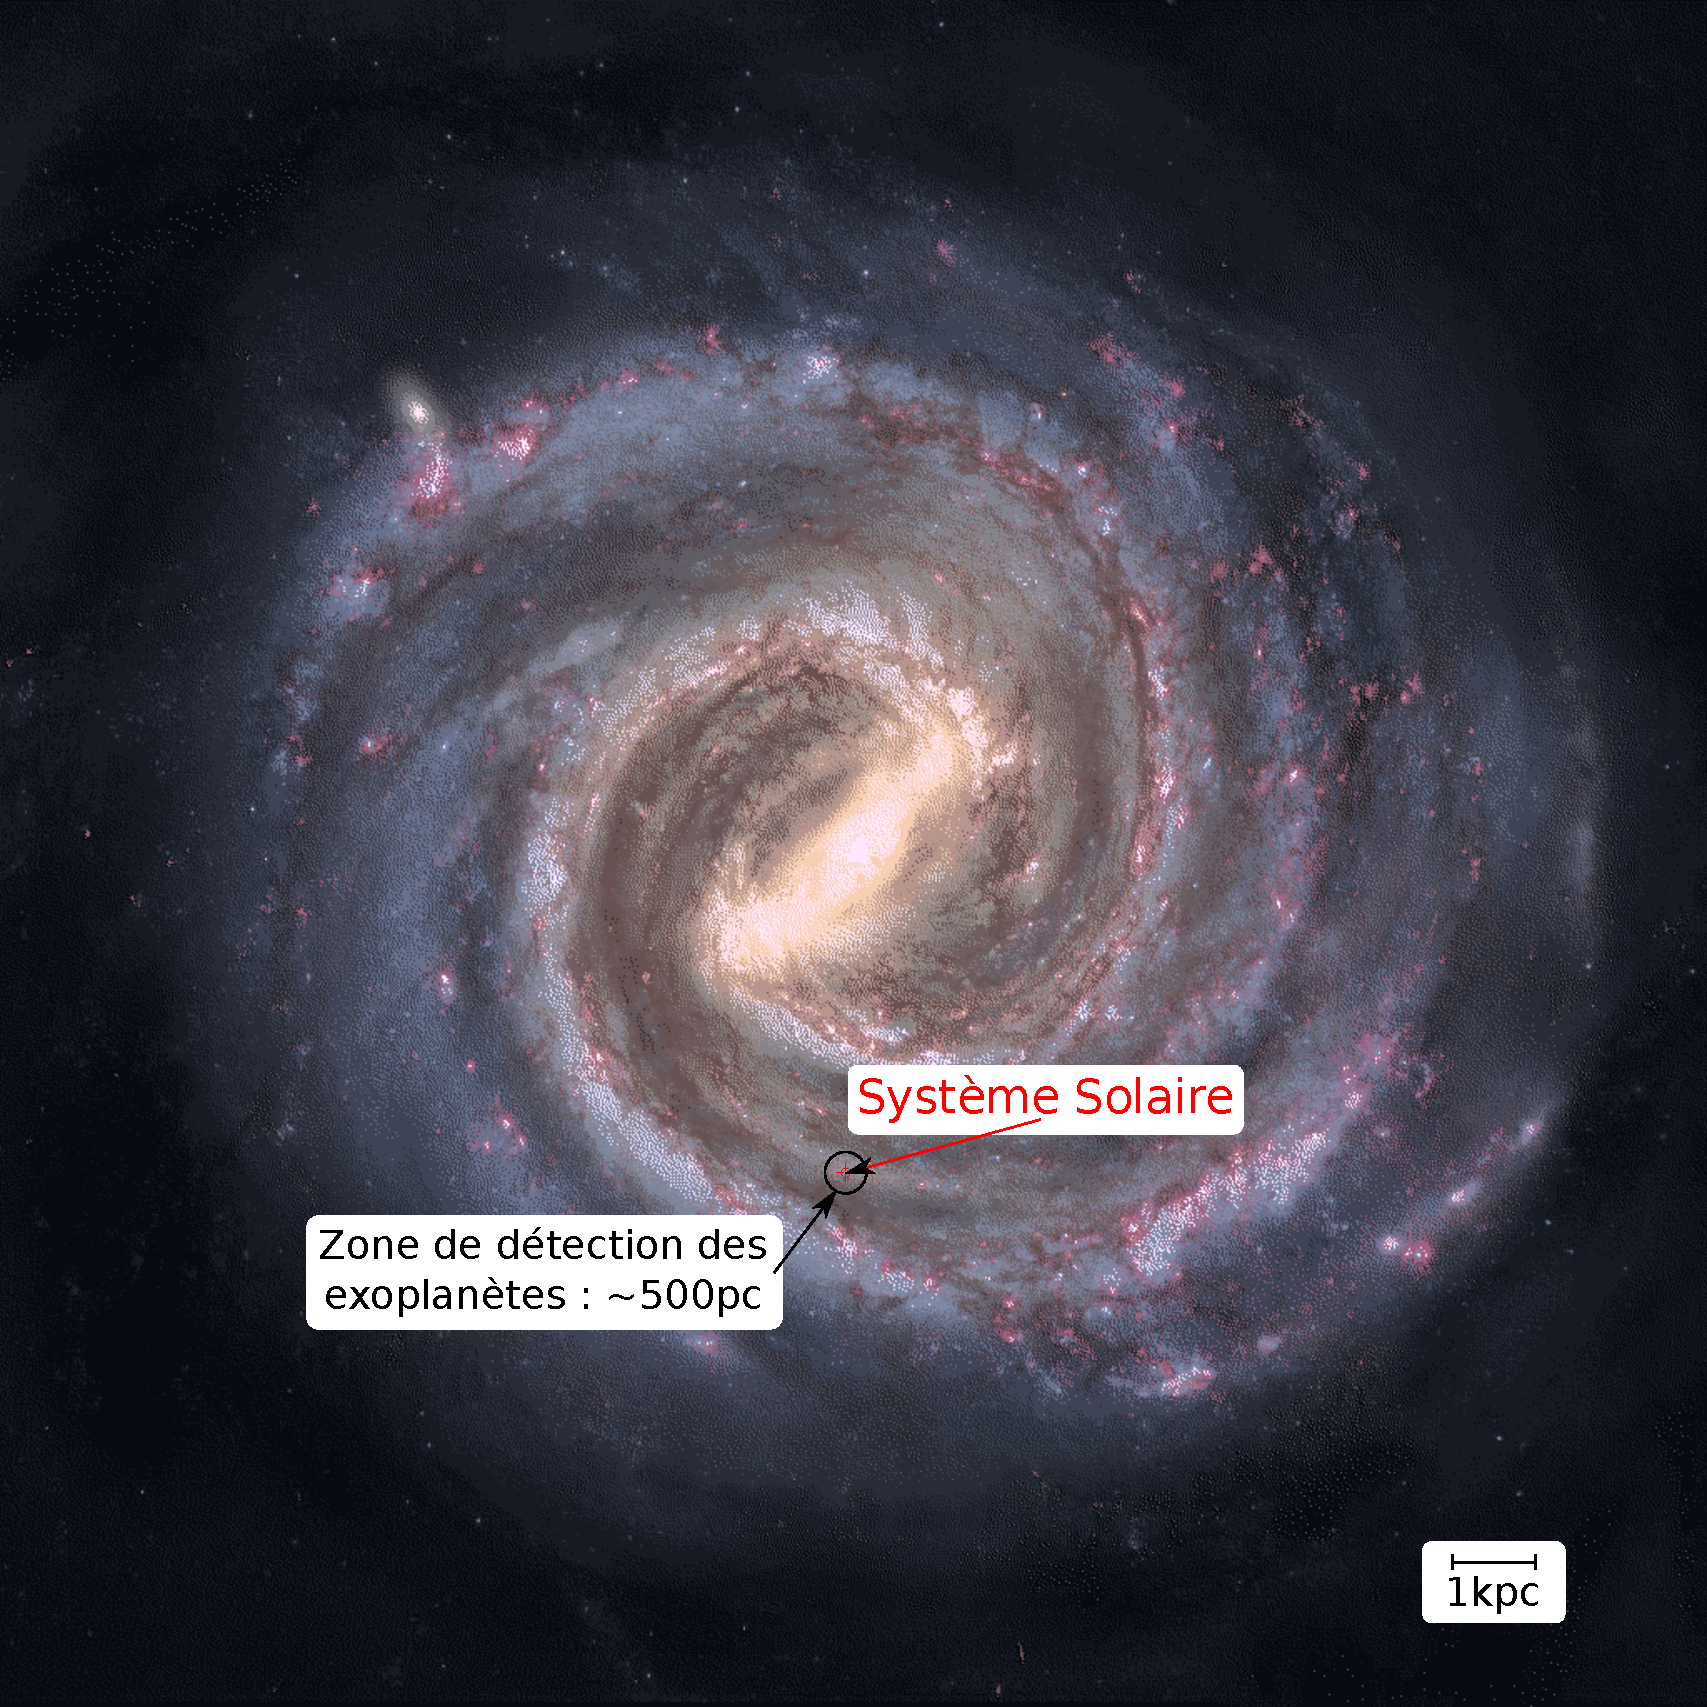
\includegraphics[width=0.45\linewidth]{figure/milky_way_exoplanets.pdf}
\caption[Sphère de détection des exoplanètes par rapport à la Voie Lactée]{Image de la voie lactée avec indication de la
position approximative du Système solaire ainsi que de la zone (en noir) contenant la majorité des exoplanètes détectées à ce
jour.}\label{fig:milky_way_exoplanet}
\end{figure}

À l'aide de différentes techniques de détection, et différents instruments dédiés, le nombre d'exoplanètes détectés à récemment fortement augmenté. Le nombre total s'élève à près de 1000 exoplanètes. Au moins autant de planètes ont été détectées mais non confirmés grâce au satellite Kepler, la liste des candidats qu'il fournit étant tellement importante qu'il est impossible de tout confirmer au fur et à mesure. Il devient
possible d'estimer la probabilité pour qu'une étoile héberge au moins une planète \citep{mayor2011road}. D'autres études
estiment même la sensibilité de cette probabilité en fonction de paramètres stellaires \citep{fischer2005planet,
johnson2007new, howard2012occurrence} ou planétaires \citep{mayor2011road, howard2010occurrence}. 

Mais le point qui me semble le plus intéressant est la découverte de types de planètes qui n'existent pas dans le système
solaire. En un mot : diversité. Que ce soient les Jupiters chauds, comme \object{51 Peg b} ou les super-Terres comme
\object{Gliese 1214 b}, ces planètes n'ont pas d'équivalent dans le Système solaire. Ces variétés de compositions, de tailles et de
systèmes nous offrent un champ de connaissance toujours plus grand dans lequel tester nos modèles de formation planétaire.
Cette diversité nous permet aussi de mieux comprendre notre propre système, comment il s'est formé, et surtout de le mettre
en perspective par rapport à tous les autres systèmes planétaires que nous observons maintenant.

Les planètes géantes, en raison de leur masse importante, ont une influence majeure sur la dynamique du système planétaire tout entier. À ce titre, il est donc primordial de comprendre leur formation, qui doit avoir lieu très tôt dans la vie du disque. En effet, ces planètes possèdent une enveloppe d'hydrogène et d'hélium qu'on ne peut expliquer sans la présence du disque de gaz au moment de leur formation. Deux modèles principaux permettent d'expliquer leur formation. Dans le premier, les planètes géantes se forment par instabilité gravitationnelle dans le disque protoplanétaire \citep{boss1997giant}. Dans un deuxième modèle \citep{pollack1996formation, alibert2004migration, levison2010modeling}, il se forme d'abord un cœur rocheux de plusieurs masses terrestres puis, dans un deuxième temps, ce cœur rocheux va accréter une enveloppe de gaz à partir du disque toujours présent. 

Une fois les planètes géantes formées, seules les planètes telluriques restent à former, ces dernières mettant beaucoup plus de temps à terminer cette phase \citep{morbidelli2012building}. Ici, les embryons de planètes telluriques sont fortement influencés par les planètes géantes et leur évolution. 

Le modèle d'accrétion de cœur est devenu le modèle privilégié lors de l'étude de la formation des planètes géantes. Ça n'exclue pas pour autant que certaines planètes géantes se forment par instabilité gravitationnelle. 

Ici, je ne vais considérer que le modèle d'accrétion de cœur pour étudier un aspect particulier de la formation planétaire. Un type particulier de planète a aiguisé mon intérêt, ce sont les super-Terres ($1$ - $10\mearth$) : parce
qu'elles sont rocheuses, à la fois semblables et différentes de la Terre, mais aussi et surtout parce qu'il n'en existe pas dans
le système Solaire. Mon but a donc été d'imaginer des modèles dans lesquels les formations du système Solaire et des
super-Terres seraient compatibles, au sein d'un même cadre théorique.

Des modèles de formation de super-Terres existent \citep{terquem2007migration, chiang2013minimum}, mais pour l'instant, aucun d'entre eux n'est capable d'expliquer à la fois la formation des planètes géantes et des super-Terres.  En me restreignant au modèle d'accrétion de cœur, je vais étudier la formation des cœurs de planète géante et de tous les types de planètes rocheuses au sein d'un même modèle. Je vais ainsi étudier un même mécanisme de formation, mais au cours de toute la vie du disque. L'environnement dans lequel se produit la formation des cœurs rocheux va ainsi changer, s'appauvrissant en gaz au fur et à mesure de la dissipation du disque.

Dans un premier chapitre \refsec{sec:chap1}, je présenterai la physique des disques, en me concentrant sur leur formation et leur évolution, mais aussi les interactions entre ce dernier et les planètes qui se forment en son sein. Ensuite, je
présenterai les modèles numériques que j'ai utilisés \refsec{sec:chap2}. Puis je détaillerai la migration planétaire dans une
grande variété de disques protoplanétaires \refsec{sec:chap3}, variant divers paramètres clé afin d'en étudier l'influence sur
la migration. Je présenterai des mécanismes de formation planétaire \refsec{sec:chap4}, en portant une attention particulière
aux super-Terres. Enfin, je conclurai en récapitulant les résultats principaux de ma thèse et les perspectives qui en découlent
\refsec{sec:discussion}.
